\documentclass{standalone}
\usepackage{tikz}
\usetikzlibrary{patterns, positioning}
\usepackage[sfdefault]{ClearSans} %% option 'sfdefault' activates Clear Sans as the default text font
\usepackage[T1]{fontenc}

\begin{document}
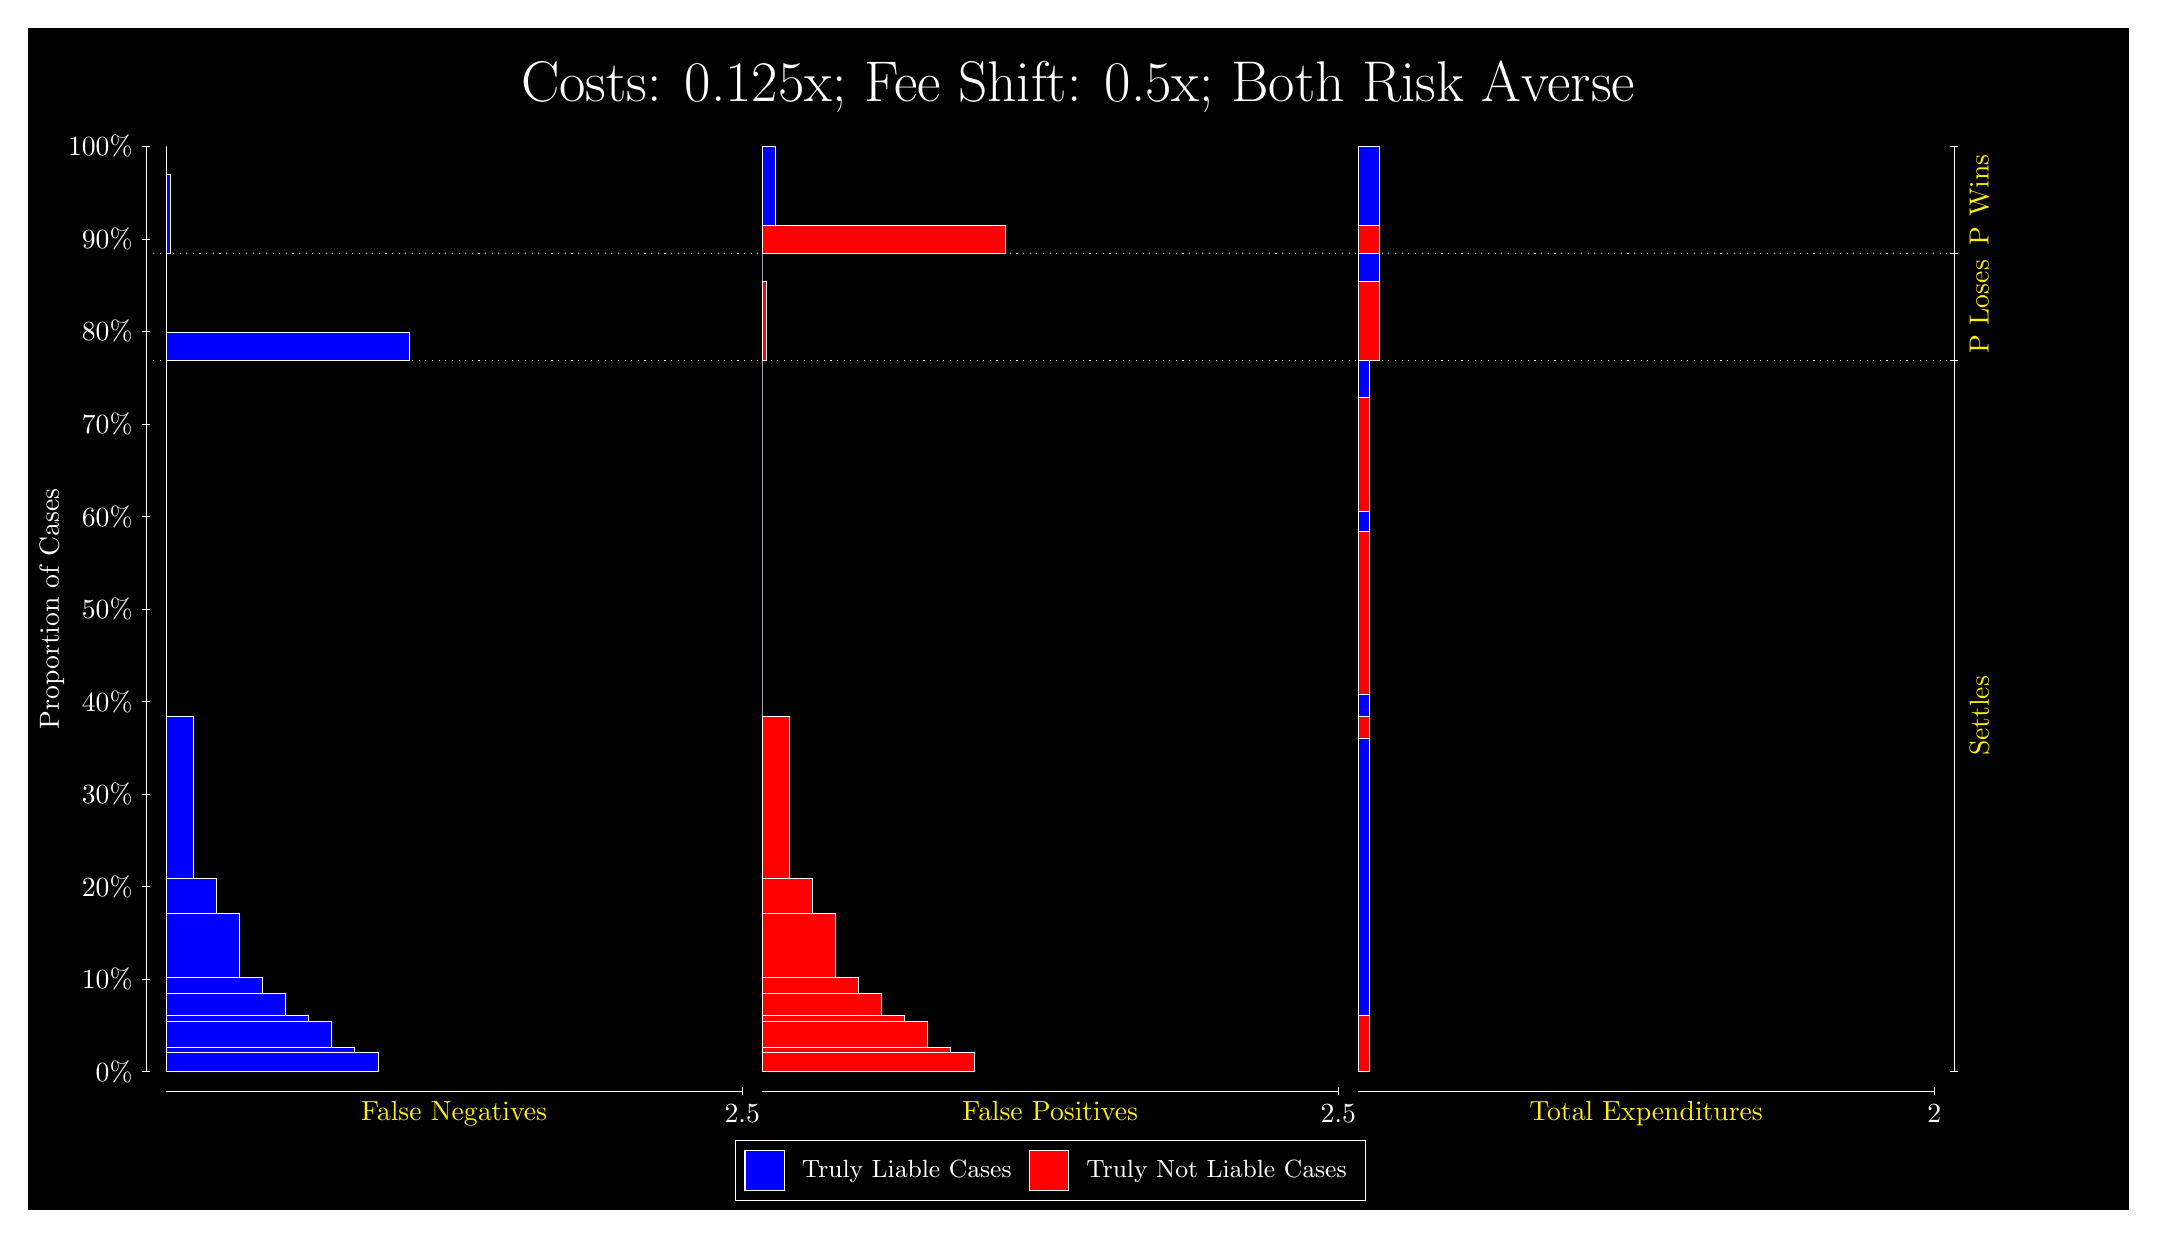
\begin{tikzpicture}
\draw[fill=black] (0,0) rectangle (26.667,15);
\draw[text=white] (0,13.5) rectangle (26.667,15) node[midway] {\huge Costs: 0.125x; Fee Shift: 0.5x; Both Risk Averse};
\draw[white, very thin] (1.5,1.75) -- (1.5,13.5);
\node[rotate=90, text=white, anchor=center] at (0.3, 7.625) {Proportion of Cases};
\draw[white, very thin] (1.45,1.75) -- (1.55,1.75);
\node[text=white, anchor=east] at (1.45, 1.75) {0\%};
\draw[white, very thin] (1.45,2.925) -- (1.55,2.925);
\node[text=white, anchor=east] at (1.45, 2.925) {10\%};
\draw[white, very thin] (1.45,4.1) -- (1.55,4.1);
\node[text=white, anchor=east] at (1.45, 4.1) {20\%};
\draw[white, very thin] (1.45,5.275) -- (1.55,5.275);
\node[text=white, anchor=east] at (1.45, 5.275) {30\%};
\draw[white, very thin] (1.45,6.45) -- (1.55,6.45);
\node[text=white, anchor=east] at (1.45, 6.45) {40\%};
\draw[white, very thin] (1.45,7.625) -- (1.55,7.625);
\node[text=white, anchor=east] at (1.45, 7.625) {50\%};
\draw[white, very thin] (1.45,8.8) -- (1.55,8.8);
\node[text=white, anchor=east] at (1.45, 8.8) {60\%};
\draw[white, very thin] (1.45,9.975) -- (1.55,9.975);
\node[text=white, anchor=east] at (1.45, 9.975) {70\%};
\draw[white, very thin] (1.45,11.15) -- (1.55,11.15);
\node[text=white, anchor=east] at (1.45, 11.15) {80\%};
\draw[white, very thin] (1.45,12.325) -- (1.55,12.325);
\node[text=white, anchor=east] at (1.45, 12.325) {90\%};
\draw[white, very thin] (1.45,13.5) -- (1.55,13.5);
\node[text=white, anchor=east] at (1.45, 13.5) {100\%};

\draw[white, very thin] (24.457,1.75) -- (24.457,13.5);
\draw[white, very thin] (24.407,1.75) -- (24.507,1.75);
\node[anchor=west] at (24.407, 1.75) {};
\draw[white, very thin] (24.407,10.784) -- (24.507,10.784);
\node[anchor=west] at (24.407, 10.784) {};
\draw[white, very thin] (24.407,12.142) -- (24.507,12.142);
\node[anchor=west] at (24.407, 12.142) {};
\draw[white, very thin] (24.407,13.5) -- (24.507,13.5);
\node[anchor=west] at (24.407, 13.5) {};

\draw[white, very thin, fill=blue] (1.75,1.75) rectangle (4.4397,1.9979);
\draw[white, very thin, fill=blue] (1.75,1.9979) rectangle (4.1469,2.0551);
\draw[white, very thin, fill=blue] (1.75,2.0551) rectangle (3.8542,2.3843);
\draw[white, very thin, fill=blue] (1.75,2.3843) rectangle (3.5614,2.4661);
\draw[white, very thin, fill=blue] (1.75,2.4661) rectangle (3.2687,2.7453);
\draw[white, very thin, fill=blue] (1.75,2.7453) rectangle (2.9759,2.9494);
\draw[white, very thin, fill=blue] (1.75,2.9494) rectangle (2.6832,3.7561);
\draw[white, very thin, fill=blue] (1.75,3.7561) rectangle (2.3904,4.2);
\draw[white, very thin, fill=blue] (1.75,4.2) rectangle (2.0976,6.2671);
\draw[white, very thin, fill=red] (1.75,6.2671) rectangle (1.75,10.784);
\draw[white, very thin, fill=blue] (1.75,10.784) rectangle (4.8422,11.134);
\draw[white, very thin, fill=red] (1.75,11.134) rectangle (1.75,12.142);
\draw[white, very thin, fill=blue] (1.75,12.142) rectangle (1.8049,13.15);
\draw[white, very thin, fill=red] (1.75,13.15) rectangle (1.75,13.5);
\draw[white, very thin, fill=red] (9.3189,1.75) rectangle (12.009,1.9979);
\draw[white, very thin, fill=red] (9.3189,1.9979) rectangle (11.716,2.0551);
\draw[white, very thin, fill=red] (9.3189,2.0551) rectangle (11.423,2.3843);
\draw[white, very thin, fill=red] (9.3189,2.3843) rectangle (11.13,2.4661);
\draw[white, very thin, fill=red] (9.3189,2.4661) rectangle (10.838,2.7453);
\draw[white, very thin, fill=red] (9.3189,2.7453) rectangle (10.545,2.9494);
\draw[white, very thin, fill=red] (9.3189,2.9494) rectangle (10.252,3.7561);
\draw[white, very thin, fill=red] (9.3189,3.7561) rectangle (9.9593,4.2);
\draw[white, very thin, fill=red] (9.3189,4.2) rectangle (9.6665,6.2672);
\draw[white, very thin, fill=blue] (9.3189,6.2672) rectangle (9.3189,10.784);
\draw[white, very thin, fill=red] (9.3189,10.784) rectangle (9.3738,11.792);
\draw[white, very thin, fill=blue] (9.3189,11.792) rectangle (9.3189,12.142);
\draw[white, very thin, fill=red] (9.3189,12.142) rectangle (12.411,12.492);
\draw[white, very thin, fill=blue] (9.3189,12.492) rectangle (9.4835,13.5);
\draw[white, very thin, fill=red] (16.888,1.75) rectangle (17.025,2.4661);
\draw[white, very thin, fill=blue] (16.888,2.4661) rectangle (17.025,5.9878);
\draw[white, very thin, fill=red] (16.888,5.9878) rectangle (17.025,6.267);
\draw[white, very thin, fill=blue] (16.888,6.267) rectangle (17.025,6.5462);
\draw[white, very thin, fill=red] (16.888,6.5462) rectangle (17.025,8.6134);
\draw[white, very thin, fill=blue] (16.888,8.6134) rectangle (17.025,8.8613);
\draw[white, very thin, fill=red] (16.888,8.8613) rectangle (17.025,10.316);
\draw[white, very thin, fill=blue] (16.888,10.316) rectangle (17.025,10.784);
\draw[white, very thin, fill=red] (16.888,10.784) rectangle (17.162,11.792);
\draw[white, very thin, fill=blue] (16.888,11.792) rectangle (17.162,12.142);
\draw[white, very thin, fill=red] (16.888,12.142) rectangle (17.162,12.492);
\draw[white, very thin, fill=blue] (16.888,12.492) rectangle (17.162,13.5);
\draw[white, dotted] (1.5,10.784) -- (24.457,10.784);
\draw[white, dotted] (1.5,12.142) -- (24.457,12.142);
\draw[white, very thin] (1.75,1.5) -- (9.0689,1.5);
\node[text=yellow, anchor=north] at (5.4094, 1.5) {False Negatives};
\draw[white, very thin] (9.0689,1.45) -- (9.0689,1.55);
\node[text=white, anchor=north] at (9.0689, 1.45) {2.5};

\draw[white, very thin] (9.3189,1.5) -- (16.638,1.5);
\node[text=yellow, anchor=north] at (12.978, 1.5) {False Positives};
\draw[white, very thin] (16.638,1.45) -- (16.638,1.55);
\node[text=white, anchor=north] at (16.638, 1.45) {2.5};

\draw[white, very thin] (16.888,1.5) -- (24.207,1.5);
\node[text=yellow, anchor=north] at (20.547, 1.5) {Total Expenditures};
\draw[white, very thin] (24.207,1.45) -- (24.207,1.55);
\node[text=white, anchor=north] at (24.207, 1.45) {2};

\node[text=yellow, centered, rotate=90] at (24.777, 6.2671) {Settles};
\node[text=yellow, centered, rotate=90] at (24.777, 11.463) {P Loses};
\node[text=yellow, centered, rotate=90] at (24.777, 12.821) {P Wins};

\draw (12.978300999999998,1.5) node[draw=none] (baseCoordinate) {};
\begin{scope}[align=center]
        \matrix[scale=0.5, draw=white, below=0.5cm of baseCoordinate, nodes={draw}, column sep=0.1cm]{
            \node[rectangle, draw, minimum width=0.5cm, minimum height=0.5cm, fill=blue] {}; &
            \node[draw=none, font=\small, text=white] (B) {Truly Liable Cases}; &
            \node[rectangle, draw, minimum width=0.5cm, minimum height=0.5cm, fill=red] {}; &
            \node[draw=none, font=\small, text=white] (B) {Truly Not Liable Cases}; \\
            };
\end{scope}

\end{tikzpicture}
\end{document}